\chapter{Linear connections}

\section{Linear connection}\label{chap2:sec1}\pageoriginale

\subsection{}\label{chap2:2.1.1}

\begin{defi*}
From \ref{chap0:0.4.9} we see that, for $x$ in $T(M)$, if $H_{x}$ is
transverse to $V_{x}$ (i.e. a supplement to $V_{x}$ in $T_{x}(T(M))$
then the restriction
$$
p^{T}|H_{x}:H_{x}\to T_{p}(x)(M)
$$
is an isomorphism. So a natural question is whether it is possible to
choose an interesting map $x\to H_{x}$ where $x$ runs through $M$. For
an open subset $A$ of $\mathbb{R}^{d}$ we see that the choice
\begin{equation*}
H_{x}=(\zeta^{T}_{x})^{-1}(0)\tag{2.1.2}\label{chap2:2.1.2}
\end{equation*}
gives us such a distribution of $H_{x}$. We look upon such a choice as
a map
\begin{equation*}
\mathcal{C}:T(M)\mathop{\times}_{M}T(M)\ni (x,y)\to
\mathcal{C}(x,y)\in T(T(M)).\tag{2.1.3}\label{chap2:2.1.3}
\end{equation*}
where $x$ determines the fibre containing $H_{x}$ and $y$, by means of
the inverse of the isomorphism $(p^{T}|H_{x}):H_{x}\to T_{p(y)}(M)$,
the element $\mathcal{C}(x,y)$ in $H_{x}$ such that
$p^{T}(\mathcal{C}(x,y))=y$.
\end{defi*}

Relative to $(U,r)$, with the notation of \ref{chap0:sec4} we have, by
\ref{chap2:2.1.1},
\begin{equation*}
\mathcal{C}((a,b),(a,b'))\mathop{=}_{\cup}
(a,b,b',.).\tag{2.1.4}\label{chap2:2.1.4} 
\end{equation*}

Keeping this in mind we define a {\em connection}.

\setcounter{subsection}{4}

\subsection{}\label{chap2:2.1.5} 

\begin{defi*}
A \pageoriginale connection on $T(M)$ (or a linear connection on $M$) is a
\begin{itemize}
\item[$\mathcal{C}_{0})$] $\mathcal{C}\in
  D(T(M){\displaystyle{\mathop{\times}_{M}}}T(M), T(T(M)))$
\end{itemize}
such that
\begin{itemize}
\item[$\mathcal{C}_{1})$]
  $(p,p^{T})\circ\mathcal{C}=\id|T(M){\displaystyle{\mathop{\times}_{M}}}T(M)$

\item[$\mathcal{C}_{2})$] $(\theta\cdot x+\eta\cdot x',y)=\theta\odot
  \mathcal{C}(x,y)\oplus \eta\odot \mathcal{C}(x',y)$

\item[$\mathcal{C}_{3})$] $(x,\theta\cdot y+\eta\cdot y')=\theta\cdot
  \mathcal{C}(x,y)+\eta\cdot \mathcal{C}(x,y')$.
\end{itemize}
\end{defi*}

(Note that this definition would make sense for any vector bundle.)

Now let us consider {\em the image set} $H_{x}$ of $\{x\}\times
T_{p(x)}(M)$ under $\mathcal{C}:H_{x}=\mathcal{C}(x,T_{p(x)}(M))$.

By $\mathcal{C}_{3})$ it follows that $H_{x}$ is a vector subspace of
$T_{x}(T(M))$; and from $\mathcal{C}_{1})$ that
$$
p^{T}(\mathcal{C}(x,y))=y
$$
and hence that
\begin{itemize}
\item[i)] $\mathcal{C}$ restricted to $\{x\}\times T_{p(x)}(M)$ is a
  monomorphism, and

\item[ii)] the only element common to $V_{x}$ and $H_{x}$ is zero.
\end{itemize}
Since the dimension of $T_{x}(T(M))$ is $2d$ and that of $V_{x}$ is
$d$ it follows, now, that
\begin{equation*}
T_{x}(T(M))=H_{x}+V_{x}\quad\text{(direct sum))}.\tag{2.1.6}\label{chap2:2.1.6}
\end{equation*}

Now we give the following definitions.

\setcounter{subsection}{6}

\subsection{}\label{chap2:2.1.7}

\begin{defi*}
For $x\in T(M)$, $H_{x}$ is called {\em the horizontal subspace} or
{\em the horizontal component of} $T_{x}(T(M))$ relative to the
connection $\mathcal{C}$. Generally we omit the reference to
$\mathcal{C}$.
\end{defi*}

\subsection{}\label{chap2:2.1.8}

\begin{defi*}
For \pageoriginale $x\in T(M)$ the map
\end{defi*}

\setcounter{subsection}{8}
\subsection{}\label{chap2:2.1.9}

$T_{x}(T(M))\ni z\to z-\mathcal{C}(x,p^{T}(z))\in T_{x}(T(M))$ is the
projection onto $V_{x}$ parallel to $H_{x}$.

\subsection{}\label{chap2:2.1.10}

\begin{defi*}
For $z$ in $T(T(M))$ the element
\end{defi*}

\setcounter{subsection}{10}

\subsection{}\label{chap2:2.1.11}

$\mathscr{U}(z)=\xi (z-\mathcal{C}(p'(z),p^{T}(z)))$ is called the
           {\em vertical component of $z$.}

\subsection{}\label{chap2:2.1.12}

\begin{note*}
From the very definition we have
$$
p\circ \mathscr{U}=p\circ p'.
$$
\end{note*}


\subsection{}\label{chap2:2.1.13}

\begin{remark*}
By $\mathcal{C}_{1})$ we have the following equations:

For $(x,y)\in T(M){\displaystyle{\mathop{\times}_{M}}}T(M)$,
\begin{align*}
p^{T}(\mathcal{C}(x,y)) &= y=p'(\mathcal{C}(y,x))\\
\text{and}\qquad p^{T}(\mathcal{C}(y,x)) &= x=p'(\mathcal{C}(x,y)).
\end{align*}
They show that the condition
$\mathcal{C}(x,y)=\overline{\mathcal{C}(y,x)}$ is compatible with
$\mathcal{C}_{1})$, $\mathcal{C}_{2})$, $\mathcal{C}_{3})$.
\end{remark*}

In view of the above, the following definition makes sense:

\subsection{}\label{chap2:2.1.14}

\begin{defi*}
A connection $\mathcal{C}$ is called {\em symmetric} if 
\end{defi*}

\setcounter{subsection}{14}
\subsection{}\label{chap2:2.1.15}
$\mathcal{C}_{4})$
$\mathcal{C}(x,y)=\overline{\mathcal{C}(y,x)} \, \forall (x,y)\in
T(M){\displaystyle{\mathop{\times}_{M}}}T(M)$ 

\medskip
\noindent
{\bf Examples.}

\setcounter{subsection}{15}
\subsection{}\label{chap2:2.1.16}
The {\em canonical connection} on an open subset $A\subset
\mathbb{R}^{d}$ is defined by
\begin{equation*}
H_{x}=(\zeta^{T}_{x})^{-1}(0)\tag{2.1.17}\label{chap2:2.1.17}
\end{equation*}
i.e.:
$$
C((a,b),(a,c))=(a,b,c,0)\quad \forall a\in A,\forall b, c\in \mathbb{R}^{d}.
$$
From \pageoriginale \ref{chap0:sec4} one sees $\mathcal{C}_{1})$,
$\mathcal{C}_{2})$, $\mathcal{C}_{3})$ and $\mathcal{C}_{4})$ are
fulfilled so that this canonical connection is moreover symmetric.

\setcounter{subsection}{17}
\subsection{}\label{chap2:2.1.18}
If $f:M\to N$ is a diffeomorphism and $C$ a connection on $N$, then
$(x,y)\to ((f^{-1})^{T})^{T}\mathcal{C}(f^{T}(x),f^{T}(y))$ defines a
connection on $M$.

\begin{exer*}
Use \ref{chap2:2.1.16}, \ref{chap2:2.1.18} and partitions of unity to build up
a connection on any manifold (a proof of that would follow also from
\ref{chap5:5.1.1}. 
\end{exer*}

\setcounter{subsection}{18}

\subsection{}\label{chap2:2.1.19}

\begin{remark*}
If $\mathcal{C}$ is a connection on $T(M)$ then
$G(x)=\mathcal{C}(x,x)$ for every $x$ in $T(M)$ is a spray, for
\begin{itemize}
\item[i)]
  $p'(G(x))=p'(\mathcal{C}(x,x))=x=p^{T}(\mathcal{C}(x,x))=p^{T}(G(x))$
  and

\item[ii)] $(G\circ h_{\theta})(x)=G(\theta\cdot x)=\mathcal{C}(\theta
  x,\theta x)=$ by \ref{chap0:0.4.21}
\begin{align*}
&= \theta\odot \mathcal{C}(x,\theta,x)=h^{T}_{\theta}(\theta\cdot
  \mathcal{C}(x,x))=\\
&= \theta\cdot h^{T}_{\theta}(\mathcal{C}(x,x))=(\theta\cdot
  (h^{T}_{\theta}\circ G))(x).
\end{align*}
This spray is called {\em the spray associated to the} given connection.
\end{itemize}
\end{remark*}

\subsection{}\label{chap2:2.1.20}

\begin{claim*}
For an open subset $A\subset \mathbb{R}^{d}$ the geodesics relative to
the spray associated to the canonical connection are open segments of
straight lines.
\end{claim*}

With the above notation, the definition shows that $f$ is a geodesic
if and only if
$$
f''-G\circ f'=0,
$$
i.e. if and only if
$f''-\mathcal{C}(p'(f''),p^{T}(f''))=0$. By\pageoriginale the
definition of canonical connection $C$ and being horizontal we have 
\begin{equation*}
\zeta^{T}(C(p'(f''),p^{T}(f''))=0.\tag{2.1.21}\label{chap2:2.1.21}
\end{equation*}
Hence, by \eqref{chap2:2.1.21}, (\ref{chap0:0.4.20}) and (\ref{chap0:0.5.9}) $f$
is a geodesic if and only if
\begin{equation*}
\zeta^{T}(f'')=0.\tag{2.1.22}\label{chap2:2.1.22}
\end{equation*}
But
$$
\zeta^{T}(f'')=\zeta^{T}\circ {f'}^{T}\circ P=(\zeta\circ f')^{T}\circ
P=\dfrac{d}{\dt}(\zeta\circ f')
$$
Hence $f$ is a geodesic if and only if $\dfrac{d(\zeta\circ
  f)}{\dt}=0$, i.e. if and only if $\zeta\circ f'=x$, a constant
vector.

But then
$$
f(t)=tx+y\quad\text{(for suitable values of $t$).}
$$

\section{Connection in terms of the local coordinates}\label{chap2:sec2}

With the notation of \ref{chap0:sec4} let
$x{\displaystyle{\mathop{=}_{\cup}}}(a,b)$ and
$y{\displaystyle{\mathop{=}_{\cup}}}(a,c)$. Then $(x,y)\in\unskip\break
T(M){\displaystyle{\mathop{\times}_{M}}}T(M)$. Now given a connection
$\mathcal{C}$ on $T(M)$ we have, by (\ref{chap2:2.1.5}).

\subsection{}\label{chap2:2.2.1}
$\mathcal{C}(x,y)=(a,b,c,\delta(a,b,c))$ where $\delta$ depends on
$\mathcal{C}$, and then $\mathcal{C}_{0})$ becomes
\begin{equation*}
\delta\in D(r(U)\times \mathbb{R}^{d}\times
\mathbb{R}^{d},\mathbb{R}^{d}).\tag{2.2.2}\label{chap2:2.2.2}
\end{equation*}
Now $\mathcal{C}_{2})$ and $\mathcal{C}_{3})$ together mean that the
restriction of $\delta$ to $\{m\}\times \mathbb{R}^{d}\times
\mathbb{R}^{d}$ for $m$ in $r(U)$ is bilinear. Further $\mathcal{C}$
is symmetric if and only if $\delta$ restricted to
$\{a\}\times\mathbb{R}^{d}\times \mathbb{R}^{d}$ is (see
(\ref{chap0:0.4.19})). Now we prove a theorem which completes the remark
(\ref{chap2:2.1.19}). 

\setcounter{subsection}{2}
\subsection{}\label{chap2:2.2.3}


\begin{theorem*}[\cite{2}, th. 2, p.~173]
Given \pageoriginale a spray $G$ on $M$ there exists a unique symmetric
connection $\mathcal{C}$ on $T(M)$ such that
$$
\mathcal{C}(x,x)=G(x).
$$
\end{theorem*}

\begin{proof}
In view of the first paragraph of this article, locally, the problem
can be stated as follows:

Given a $\psi\in D(r(U)\times\mathbb{R}^{d},\mathbb{R}^{d})$ such that
for a fixed $m$ in $r(U)$, $\psi$ is a quadratic form in the other
variable to construct a $\delta\in D(r(U)\times\mathbb{R}^{d}\times
\mathbb{R}^{d},\mathbb{R}^{d})$ which, for fixed $m$ in $r(U)$, is
bilinear and symmetric in other variables and to prove its
uniqueness. This has been done in (\ref{chap1:1.3.3}). The uniqueness of
$\delta$ shows that the problem is local.
\end{proof}


\subsection{}\label{chap2:2.2.4}

\begin{remark*}
Let us write down $\mathcal{C}$ explicitly in terms of $G$. By
(\ref{chap0:0.4.17}) it is enough to express $\mathcal{C}$ in terms of
$G$ on $d\phi$ for $\phi\in F(M)$. We have
\begin{align*}
G(x+y)(d\phi) &=
\mathcal{C}(x+y,x+y)(d\phi)=\mathcal{C}(x+y,x)(d\phi)+\\
&\hspace{3cm} +\mathcal{C}(x+y,y)(d\phi)=\\
&=(C(x,y)\oplus\mathcal{C}(x,x))(d\phi)+(C(x,y)\oplus C(y,y))(d\phi)=\\
&=C(x,y)(d\phi)+C(y,x)(d\phi)+C(x,x)(d\phi)+\mathcal{C}(y,y)(d\phi)=\\
&\hspace{5cm} \text{by (\ref{chap0:0.4.19}), (3)}\\
&= C(x,y)(d\phi)+C(x,y)(d\phi)+G(x)(d\phi)+G(y)(d\phi)=\\
&\qquad \text{since $C$ is symmetric}\\
&= 2\mathcal{C}(x,y)(d\phi)+G(x)(d\phi)+G(y)(d\phi)\quad\text{by
  (\ref{chap0:0.4.22}).} 
\end{align*}
Hence \pageoriginale
\begin{equation*}
\mathcal{C}(x,y)(d\phi)=\frac{1}{2}\left[G(x+y)-G(x)-G(y)\right]\quad
(d\phi) \tag{2.2.5}\label{chap2:2.2.5}
\end{equation*}
which shows, once again, the uniqueness (\ref{chap0:0.4.17}).
\end{remark*}

\section{Covariant derivation}\label{chap2:sec3}

\quad For the rest of this chapter we suppose given a manifold $M$
with a connection $\mathcal{C}$. 

\subsection{}\label{chap2:2.3.1}

\begin{defi*}
Given a manifold $N$, an $X\in\mathscr{C}(N)$ and $g\in D(N,T(M))$,
the map $N\to T(M)$ defined by
\begin{equation*}
D_{X}g=\mathscr{U}\circ g^{T}\circ X \tag{2.3.2}\label{chap2:2.3.2}
\end{equation*}
is called {\em the covariant derivative of $g$ with respect to $X$.}
If $x\in T(N)$ we write $D_{x}g=\mathcal{U}(g^{T}(x))$.

\begin{center}
\begin{minipage}[c]{6cm}
%\vcenter{\xymatrix{
% & g^{T}(x)\\
%g(x)\ar@{.}[u]\ar[ur] & \\
%   & C(g(x),p^{T}(g^{T}(x))\ar[uu]\\
%O_{m}\ar@{x->}[uu]\ar[ur]& 
%}}
\begin{figure}[H]
\centering
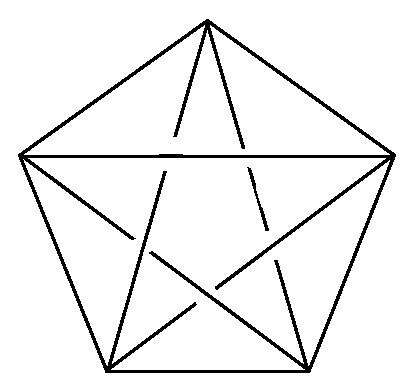
\includegraphics{chap2-fig1.eps}
\end{figure}
\end{minipage}
\begin{minipage}[c]{6cm}
\[
\xymatrix@=2cm{
 & T(T(M))\ar@<-2.5pt>[d]_{p'}\ar@<2.5pt>[d]^{\mathscr{U}}\\
T(N)\ar[ur]^{g^{T}} & T(M)\ar[d]^{p}\\
N\ar[u]^{X}\ar@<2.5pt>[ur]^{D\times g}\ar@<-2.5pt>[ur]_{g}\ar[r]_{p\circ g} & M
}
\]
\end{minipage}
\end{center}
\end{defi*}

\setcounter{subsection}{2}
\subsection{}\label{chap2:2.3.3}

\begin{remarks*}
Since $X$, $g^{T}$ and $\mathcal{U}$ are differentiable we have
$$
D_{X}g\in D(N,T(M)).
$$
\end{remarks*}


\subsection{}\label{chap2:2.3.4}

We \pageoriginale have
\begin{align*}
p\circ D_{X}g &= p\circ \mathscr{U}\circ g^{T}\circ X=\\
              &= p\circ p'\circ g^{T}\circ X\quad
                 \text{by \ (\ref{chap2:2.1.12})} =\\
              &= p\circ g
\end{align*}
and hence if $g$ is a lift of $f$ then $D_{X}g$ is again a lift of $f$.

\subsection{}\label{chap2:2.3.5}
Let $f\in D(I,M)$. Then $f^{T}$ can be considered as a map from $I$ to
$T(M)$. Now we have: $f$ is a geodesic for the spray $G$ associated to
the connection $\mathcal{C}$ if and only if 
$$
D_{P}f'=0.
$$

For we have
\begin{align*}
D_{P}f' &= \mathscr{U}\circ {f'}^{T}\circ T_{P}=\mathscr{U}\circ
f''=\xi (f''-\mathcal{C}(f',f'))=\\
        &= \xi (f''-G\circ f'),\text{ \ and \ }\quad \xi \text{ \ is an
  isomorphism}
\end{align*}
between the vertical vectors at a point and the tangent space
containing that point.

Writing $f=p\circ g$ we have
\begin{align*}
D_{X}g &= \xi(g^{T}\circ X-C(p'\circ g^{T}\circ X, p^{T}\circ
g^{T}\circ X))\tag{2.3.6}\label{chap2:2.3.6}\\
       &=\xi(g^{T}\circ X-\mathcal{C}(g,f^{T}\circ X)).
\end{align*}
Now considering an $\omega$ in $\mathcal{E}^{1}(M)$ as a linear
function on $T(M)$ and observing that $g^{T}\circ
X-\mathcal{C}(g,f^{T}\circ X)$ is vertical we obtain, by
(\ref{chap0:0.4.16}) \pageoriginale
\begin{align*}
\omega(D_{X}g) &= (g^{T}\circ X-\mathcal{C}(g,f^{T}\circ
X))(\omega)=\\
               &= X(\omega\circ g)-\mathcal{C}(g,f^{T}\circ
X)(\omega).\tag{2.3.7}\label{chap2:2.3.7} 
\end{align*}

In particular, for $\omega=d\phi$, where $\phi\in F(M)$,
\begin{equation*}
d\phi(D_{X}g)=X(d\phi\circ g)-(g,f^{T}\circ X)(d\phi).\tag{2.3.8}\label{chap2:2.3.8}
\end{equation*}

Sometimes we write $D_{X}g(\phi)$ for $d\phi(D_{X}g)$ and $X(g(\phi))$
for $X(d\phi\circ g)$.


\setcounter{subsection}{8}
\subsection{}\label{chap2:2.3.9}

\begin{examples*}
For an open subset $A\subset \mathbb{R}^{d}$ with respect to the
canonical connection we have
\begin{align*}
\nu = \zeta^{T}.\\
\text{For}\quad \nu(z) &= \nu(a,b,c,d)\tag{2.3.10}\label{chap2:2.3.10}\\
&= \xi(z-\mathcal{C}(p'(z),p^{T}(z)))\\
&= \xi ((a,b,c,d)-(a,b,c,0))=\xi(a,b,o,d)=d.
\end{align*}
and $\zeta^{T}(a,b,c,d)=d$. Hence
$$
D_{X}g=\nu\circ g^{T}\circ X=\zeta^{T}\circ g^{T}X=(\zeta\circ
g)^{T}\circ X
$$
where $g\in D(A,T(A))$.
\end{examples*}

\setcounter{subsection}{10}
\subsection{}\label{chap2:2.3.11}
In case $f=p\circ g$ is a constant map, i.e. in case $f(y)=m$ for
every $y$ in $N$, $g$ can be considered as a map from $N$ to
$T_{m}(M)$, and in this case $\nu=\zeta$. Hence we have
$$
D_{X}g=\nu\circ g^{T}X=\zeta\circ g^{T}\circ X=dg\circ X
$$
and so $D_{X}g$ is nothing but the restriction of the differential map
of \pageoriginale $g$ to the subset $\{X(y)\}$ of $T(N)$ In particular
if $g$ is a 
curve in $T_{m}(M)$, and $X=P$ on $\mathbb{R}$ we have
$$
D_{P}g=\dfrac{dg}{\dt}
$$
and hence $D_{P}g$ is the ordinary derivative of a vector valued
function.

\setcounter{subsection}{11}
\subsection{}\label{chap2:2.3.12}
If $f\in D(N,M)$ and $X$, $Y\in \mathscr{C}(N)$ then $f^{T}\circ Y\in
D(N,T(M))$ and by \eqref{chap2:2.3.8} we have
\begin{equation*}
D_{x}(f^{T}\circ Y)(\phi)=X(Y(\phi\circ f))-\mathcal{C}(f^{T}\circ
Y,f^{T}\circ X)(d\phi)\,\forall \phi\in F(M).\tag{2.3.13}\label{chap2:2.3.13}
\end{equation*}

\setcounter{subsection}{13}
\subsection{}\label{chap2:2.3.14}
For $f\in D(N,M)$, $X\in \mathscr{C}(N)$, $Y\in \mathscr{C}(M)$ and
$n\in N$ we have 
$$
D_{X(n)}(Y\circ f)=v(Y^{T}(f^{T}(X(n)))=D_{f^{T}(X(n))}Y.
$$

In particular if $f=\id_{M}$ and $X$, $Y\in\mathscr{C}(M)$, then
$D_{X}Y\in \mathscr{C}(M)$ and so $D$ can be considered as a mapping
$\mathscr{C}(M)\times\mathscr{C}(M)\to \mathscr{C}(M)$. For $f\in
D(N,M)$, $\psi\in F(N)$, $X$, $Y\in \mathscr{C}(N)$ and $g$, $g'\in
D(N,T(M))$ such that $p\circ g=p\circ g'$ we have
\begin{align*}
\text{C.D. 1. \quad} & D_{X}g\text{ is } F(N)-\text{linear in } X,\\
\text{C.D. 2. \quad} & D_{X}(g+g')=D_{X}g+D_{X}g'\\
\text{C.D. 3. \quad} & D_{X}(\psi
g)=X(\psi)g+\psi(D_{X}g)\tag{2.3.15}\label{chap2:2.3.15}\\
\text{C.D. 4. \quad} & D_{X}(f^{T}\circ Y)-D_{Y}(f^{T}\circ
X)=f^{T}\circ [X,Y] 
\end{align*}
{\em if $C$ is symmetric.}

\begin{proof}
\quad 
\begin{itemize}
\item[C.D.~1.] follows directly from the definition. To
  prove \pageoriginale the others, and 
for simplicity let us use the convention following \eqref{chap2:2.3.8}.

\item[C.D.~2.] For $\phi\in F(M)$ we have, setting $f=p\circ g$,
{\fontsize{9}{11}\selectfont
\begin{align*}
D_{X}(g+g')(\phi) &= X(g+g')\phi-\mathcal{C}(g+g',f^{T}\circ
X)(d\phi)\quad\text{(by \eqref{chap2:2.3.8})}\\
&= X(g(\phi)+g'(\phi))-(\mathcal{C}(g,f^{T}\circ X)\oplus
C(g',f^{T}\circ X))(d\phi)\\
&= X(g(\phi))+X(g'(\phi))-\mathcal{C}(g,f^{T}\circ
X))(d\phi)-\mathcal{C}(g',f^{T}\circ X)(d\phi)\\
&\quad \text{ by \ref{chap0:0.4.22}}.
\end{align*}}\relax

\item[C.D.~3.] \begin{tabbing}
               $D_{X}(\psi g)(\phi)$ \= = $X(\psi g)(\phi)-C(\psi\cdot
  g,f^{T}\circ x)(d\phi)=$\\[5pt]
  \> = $X(\psi\cdot g(\phi))-(\psi\odot \mathcal{C}(g,f^{T}\circ
  X))(d\phi)=$\\[5pt]
  \> = $X(\psi)g(\phi)+\psi X(g(\phi))$\\[5pt]
  \> $-\psi\cdot C(g,f^{T}\circ X)(d\phi)$, by (\ref{chap0:0.4.22})
\end{tabbing}

\item[C.D.~4.] \begin{tabbing}
\= $(D_{X}(f^{T}\circ Y)-D_{Y}(f^{T}\circ
  X))(\phi)=$\\[5pt]
  \>$=X(Y(\phi\circ f))-(f^{T}\circ Y, f^{T}\circ X)(d\phi)$\\[5pt]
  \>$-Y(X(\phi\circ f))-(f^{T}\circ X,f^{T}\circ Y)(d\phi)=$\\[5pt]
  \>$=[X,Y](\phi\circ f)$ \ because $\mathcal{C}$ is symmetric,
  and\\[5pt]
  \>\quad property 3) of the involution $-$, in (\ref{chap0:0.4.19})\\[5pt]
  \>$=(f^{T}\circ[X,Y])(\phi)=(f^{T}\circ[X,Y])(\phi)$.
\end{tabbing}
\end{itemize}
\end{proof}

\setcounter{subsection}{15}
\subsection{}\label{chap2:2.3.16}


\begin{lemma*}
For $f\in D(N,T(M))$, $X$, $Y\in\mathscr{C}(N)$ the map
$$
(X,Y,f)\to ([D_{X},D_{Y}]-D_{[X,Y]})(f)
$$
if $F(N)$ - trilinear.
\end{lemma*}

\begin{proof}
We have for $\psi\in F(N)$:
\begin{align*}
& (([D_{\psi X}, D_{Y}]-D_{[\psi X,Y]})(f)\\
& =\psi D_{X}D_{Y}f-D_{Y}(\psi D_{X}f)-D_{[\psi X,Y]}f\quad\text{and
    by C.D.~1.,}\\
&=\psi D_{X}D_{Y}f-D_{Y}(\psi D_{x}f)-\psi D_{[X,Y]}f+Y(\psi)D_{X}f=\\
&= \psi D_{X} D_{Y}f-\psi D_{Y}D_{X}f-Y(\psi)\cdot D_{X}f\\
&\qquad -D_{[X,Y]}f+Y(\psi)\cdot D_{X}f\quad\text{by C.D. 3.,}\\
&\qquad =\psi([D_{X},D_{Y}]-D_{[X,Y]})f.
\end{align*}\pageoriginale
Therefore the mapping is $F(N)$-linear in $X$ and since the mapping is
antisymmetric in $X$, $Y$ it is $F(N)$ - linear in $Y$.
\end{proof}

Applying C.D.~3. twice we obtain, by straightforward calculation
\begin{align*}
([D_{X},D_{Y}]-D_{[X,Y]})(\psi\cdot f)\\
=\psi([D_{X},D_{Y}]-D_{[X,Y]}f).
\end{align*}

\section{The derivation law}\label{chap2:sec4}

\subsection{}\label{chap2:2.4.1}
In case $X$, $Y\in \mathscr{C}(M)$ and $\phi\in F(M)$, with $N=M$,
C.D.'s can be written, respectively, as
\begin{itemize}
\item[D.L.1.] $D_{X}Y$ is $F(M)$-linear in $X$,

\item[D.L.2.] $D_{X}(Y+Y')=D_{X}Y+D_{X}Y'$

\item[D.L.3.] $D_{X}(\phi Y)=X(\phi)Y+\phi\cdot D_{X}Y$

\item[D.L.4.] $D_{X}Y-D_{Y}X=[X,Y]$ \ if \ $\mathscr{C}$ is symmetric.
\end{itemize}


\subsection{}\label{chap2:2.4.2}

Thus \pageoriginale from a connection we obtain a mapping from
$\mathscr{C}(M)\times \mathscr{C}(M)$ into $\mathscr{C}(M)$ satisfying
D.L. 1, 2, 3. Any such map is called a {\em Derivation Law in $M$.} It
is said to be {\em symmetric} (or without torsion) if D.L.4 holds for
it.

Conversely, given a derivation law in $M$ there is a connection which
induces the given derivation law (see Koszul \cite{18}: Th. 4. p. 94).

\subsection{}\label{chap2:2.4.3}

In local coordinates relative to $(U,r)$, let $\{X_{i}\}$ denote the
dual basis of $dx^{i}=d(\mathcal{U}i\circ r)$ and now let

\subsection{}\label{chap2:2.4.4}

$D_{X_{i}}X_{k}=\sum\limits_{j} \lambda^{j}_{ik}X_{j}$. Then we have
by \ref{chap2:2.3.12}
$$
(D_{X_{i}}X_{k})(x^{j})=X_{i}(X_{k}(x^{j}))-\mathcal{C}(X_{k},X_{i})(dx^{j}).
$$
But $X_{k}(x^{j})=\delta^{j}_{k}$ a constant and hence
$X_{i}(X_{k}(x^{j})))=0$.

Hence
\begin{align*}
& (D_{X_{i}}X_{k})(x^{j})=-\mathcal{C}(X_{k},X_{i})(dx^{j})\\
&
  =-\mathcal{U}^{j}(\delta(a,e_{k},e_{i}))=\Gamma^{j}_{ki}\quad\text{(see
    (\ref{chap1:1.3.4}))}. 
\end{align*}

\setcounter{subsection}{4}
\subsection{}\label{chap2:2.4.5}

Thus $\lambda^{j}_{ik}=\Gamma^{j}_{ki}$.

Given $\omega\in \mathscr{L}^{r}(M)$ and $X\in \mathscr{C}(M)$ we
define a map
$$
D\omega:\mathscr{C}^{r+1}(M)\to F(M)\quad\text{by setting}
$$

\subsection{}\label{chap2:2.4.6}

\begin{align*}
& (D\omega)(X,X_{1},\ldots\ldots,X_{r})=X(\omega(X_{1},\ldots\ldots,X_{r}))-\\
& -\sum^{r}_{i=1}\omega (X_{1},\ldots,X_{i-1},D_{X}X_{i},X_{i+1},\ldots,X_{r})
\end{align*}
$\forall X_{1},\ldots,X_{r}\in\mathscr{C}(M)$.

Then \pageoriginale we have
\begin{itemize}
\item[i)] $D\omega$ is $(r+1)$-additive

\item[ii)] $(D\omega)(\phi X,X_{1},\ldots,X_{r})=$
$$
\phi\cdot
X(\omega(X_{1},\ldots,X_{r}))-\sum^{r}_{i=1}\omega(X_{1},\ldots,X_{i-1},\phi\cdot D_{X}X_{i},X_{i+1},\ldots,X_{r})=
$$
by \ref{chap2:2.4.1} D.L.1.
$$
=\phi(D\omega)(X,X_{1},\ldots,X_{r})
$$
and

\item[iii)] $D(\omega)(X,\phi X_{1},\ldots,X_{r})=X(\omega(\phi
  X_{1},\ldots,X_{r}))$
\begin{align*}
&-(D_{X}(\phi X_{1}),X_{2},\ldots,X_{r})-\sum^{r}_{i=2}\omega(\phi
X_{1},\ldots,D_{X}X_{i},\ldots,X_{r})=\\
&=\phi
X(\omega(X_{1},\ldots,X_{r}))+(X(\phi)\omega(X_{1},X_{2},\ldots,X_{r})\\
&{}-\omega(X(\phi),X_{1},X_{2},\ldots,X_{r})
-\omega(\phi D_{X}X_{1},X_{2},\ldots,X_{r})\\
&{}-\sum^{r}_{i=2}\phi\omega(X_{1},\ldots,X_{i-1},D_{X}X_{i},X_{i+1},\ldots,X_{r})=\\
&=\phi(D\omega)(X,X_{1},\ldots,X_{2})
\end{align*}
and similarly for $i=2,\ldots,r$.
\end{itemize}

\setcounter{subsection}{6}
\subsection{}\label{chap2:2.4.7}
Hence $D\in \mathscr{L}^{r+1}(M)$. However, in general, if $\omega\in
\mathcal{E}^{r}(M)$, $D\omega$ may not belong to
$\mathcal{E}^{r+1}(M)$). This form $D\omega$ is called the {\em
  covariant derivative} of $\omega$ with the respect to $D$ or $C$
(the derivation law or the connection). More generally:

\begin{prop*}[2.4.7 bis]\label{chap2:prop2.4.7bis}
Let $X\in \mathscr{C}(N)$, $g_{1},\ldots,g_{r}\in D(N,T(M))$, $f\in
D(N,M)$ maps such that $p\circ g_{i}=f\forall i=1,\ldots,r$; and
$\omega\in \mathscr{E}^{r}(M)$. Then $(D\omega)(f^{T}\circ
X,g_{1},\ldots,g_{r})=X(\omega(g_{1},\ldots,g_{r}))-{\displaystyle{\mathop{\sum}^{r}_{i=1}}}\omega
(g_{1},\ldots,g_{i-1},\unskip\break D_{X}g_{i}, g_{i+1},\ldots,g_{r})$.
\end{prop*}

\begin{proof}
This\pageoriginale follows from the local expression of $f_{T}\circ X$
given by (\ref{chap2:2.5.14}) and linearity.
\end{proof}

Now we set
\begin{equation*}\label{chap2:2.4.8}
D_{X}\omega=i(X)\circ D\omega\tag{2.4.8}
\end{equation*}

\setcounter{subsection}{8}
\subsection{}\label{chap2:2.4.9}

\begin{prop*}
For $\omega\in\mathscr{E}^{1}(M)$ and $(x,y)\in
T(M){\displaystyle{\mathop{=}_{M}}}T(M)$ we have
$$
(D\omega)(x,y)=\mathcal{C}(y,x)(\omega).
$$
\end{prop*}

\begin{proof}
Let $X$, $Y\in\mathscr{C}(M)$ be such that
$$
X(p(x))=x\quad\text{and}\quad Y(p(y))=y.
$$
Then by \eqref{chap2:2.3.7} we have
$$
\omega(D_{X}Y)=X(\omega\circ Y)-\mathcal{C}(Y,X)(\omega)
$$
and so
\begin{gather*}
C(Y,X)(\omega)=X(\omega(Y))-\omega(D_{X}Y)=\\
=(D\omega)(X,Y)\quad\text{by the definition of } D\omega.
\end{gather*}
\end{proof}


\subsection{}\label{chap2:2.4.10}

\begin{lemma*}
With the above notation
$$
(d\omega)(x,y)=(D\omega)(x,y)-(D\omega)(y,x)
$$
provided that $\mathcal{C}$ is symmetric.
\end{lemma*}

\begin{proof}
With the same notation, we have
\begin{align*}
& (D\omega)(X,Y)-(D\omega)(Y,X)\\
&\quad =X(\omega(Y))-\omega(D_{X}Y)-Y(\omega(X))+\omega(D_{Y}(X))\\
&\quad =X(\omega(Y))-Y(\omega(X))-\omega([X,Y])
\end{align*}
since $\mathscr{C}$ is symmetric $=(d\omega)(X,Y)$\pageoriginale (by
the definition of $d\omega$: see ({\small\ref{chap0:0.2.10}})).
\end{proof}

\subsection{}\label{chap2:2.4.11}

\begin{defi*}
For $\phi\in F(M)$ $Dd\phi\in\mathscr{E}^{2}(M)$ is called {\em the
  Hessian of $\phi$} with respect to the connection $C$.
\end{defi*}


\subsection{}\label{chap2:2.4.12}

\begin{coro*}
If $C$ is symmetric then
$$
Dd\phi\quad\text{is symmetric}\quad \forall \phi\in F(M).
$$
\end{coro*}

\begin{proof}
By the above proposition we have, with the same notation,
\begin{align*}
(Dd\phi)(x,y) &= C(y,x)(d\phi)\\
&= \overline{C(y,x)}(d\phi)=C(x,y)(d\phi) \ \text{(see \ref{chap0:0.4.19}
    \& \ref{chap2:2.1.15})}=\\
&= (Dd\phi)(y,x).
\end{align*}
\end{proof}

\subsection{}\label{chap2:2.4.13}

\begin{prop*}
If $f$ is a geodesic of $M$ with respect to the spray associated to
$C$, then for $\phi\in F(M)$ we have
$$
\frac{d^{2}(\phi\circ f)}{\dt^{2}}=(Dd\phi)(f',f').
$$
\end{prop*}

\begin{proof}
The fact that $f$ is a geodesic implies that
\begin{align*}
& f'' =C(f',f')\text{ \ and hence}\\
& f''(d\phi)=C(f',f')(d\phi).\\
\text{But \ \ } & f''(d\phi)=\frac{d^{2}(\phi\circ f)}{\dt^{2}}
\ \ \text{(see \ref{chap0:0.5.10})}
\end{align*}
and by the proposition above
$$
C(f',f')(d\phi)=(Dd\phi)(f',f').
$$
\end{proof}

\section{Curvature}\label{chap2:sec5}

\subsection{}\label{chap2:2.5.1}
Let $X$, $Y\in \mathscr{C}(M)$ and let us write
$$
R(X,Y)=[D_{X},D_{Y}]-D_{[X,Y]} \ \ \text{(defect of brackets).}
$$
Then \pageoriginale by (\ref{chap2:2.3.16}) it follows that $R\in
\mathscr{L}^{3}_{1}(M)$. This map $R$ is called the curvature tensor
of $M$ for $D$.

$R$ has the following properties:

\setcounter{subsection}{1}
\subsection{}\label{chap2:2.5.2}

\begin{itemize}
\item[C.T.~1.] $R(X,Y)=-R(Y,X)$,

\item[C.T.~2.] $R(X,Y)Z+R(Y,Z)X+R(Z,X)Y=0$ if $C$ is symmetric.
\end{itemize}
The equality {\em C.T.~1.} follows from the definition of $R$, so let
us consider {\em C.T.~2.} We have in succession, applying the
definition of $R$ and {\em D.L.~4.,} \ref{chap2:2.4.1}, six times.
\begin{align*}
& R(X,Y)Z+R(Y,Z)X+R(Z,X)Y\\
& = D_{X}D_{Y}Z-D_{Y}D_{X}Z-D_{[X,Y]}Z\\
& +D_{Y}D_{Z}X-D_{Z}D_{Y}X-D_{[Y,Z]}X\\
& +D_{Z}D_{X}Y-D_{X}D_{Z}Y-D_{[Z,X]}Y=\\
& =D_{X}(D_{Y}Z-D_{Z}Y)+D_{Y}(D_{Z}X-D_{X}Z)+D_{Z}(D_{Y}X-D_{X}Y)\\
& - D_{[Y,Z]}X-D_{[Z,X]}Y-D_{[X,Y]}Z\\
&=
  D_{X}[Y,Z]-D_{[Y,Z]}X+D_{Y}[Z,X]-D_{[Z,X]}Y+D_{Z}[Y,X]-D_{[Y,X]}Z=\\
&= [X,[Y,Z]]+[Y,[Z,X]]+[Z,[XY]]
\end{align*}
which is zero by Jacobi identity in $\mathscr{C}(M)$.

\medskip
\noindent
{\bf Examples.}


\subsection{}\label{chap2:2.5.3} 
1. If the dimension of $M$ is $1$ then
  $R=0$ by {\em  C.T. 1.}

\subsection{}\label{chap2:2.5.4} 
2. For an open subset $A$ of $\mathbb{R}^{d}$ we have 
$$
R=0
$$
the \pageoriginale connection being the canonical connection. To see
this let $x$, $y$, $z$ be vectors and $X$, $Y$, $Z$ be vector fields
such that $X(m)=x$, $Y(m)=y$, and $\zeta\circ Z=\{\zeta(Z)\}$. Then we
have
$$
D_{X}Z=\nu \circ Z^{T}\circ X=\zeta^{T}\circ Z^{T}\circ X=(\zeta\circ
Z)^{T}\circ X.
$$
But $\zeta\circ Z$ is constant and hence
$$
(\zeta\circ Z)^{T}=0.
$$
This argument actually shows that
$$
D_{X}D_{Y}Z=0, D_{Y}D_{X}Z=0, D_{[X,Y]}Z=0.
$$


\setcounter{subsection}{4}
\subsection{}\label{chap2:2.5.5}

\begin{note*}
We can define the covariant derivative $D\Omega$ for any
$\Omega\in\mathscr{L}^{r}_{s}(M)$ and then for $R$ we can prove the
Bianchi identity.
\begin{equation*}
D_{X}R(Y,Z)+D_{Y}R(Z,X)+D_{Z}R(X,Y)=0\quad\text{(see
  \cite{18}).}\tag{2.5.6}\label{chap2:2.5.6} 
\end{equation*}
\end{note*}

\setcounter{subsection}{6}
\subsection{}\label{chap2:2.5.7}

\begin{lemma*}
For $\omega\in \mathscr{E}^{1}(M)$, $X$, $Y$, $Z\in \mathscr{C}(M)$:
$$
([D_{X},D_{Y}]-D_{[X,Y]})\omega=-R(X,Y)\cdot \omega
$$
\end{lemma*}

\begin{proof}
For any $Z\in \mathscr{C}(M)$ the left hand side, by definition
\ref{chap2:2.4.6}, is equal to
\begin{align*}
& (D_{X}D_{Y}\omega)(Z)-(D_{Y}D_{X}\omega)(Z)-(D_{[X,Y]}\omega)(Z)\\
& =X(D_{Y}\omega)(Z))-(D_{Y}\omega)(D_{X}Z)-Y((D_{X}\omega))(Z))\\
& +(D_{X}\omega)(D_{Y}Z)-[X,Y](\omega(Z))+\omega(D_{[X,Y]}Z)\\
& =X(Y(\omega(Z)))-X(\omega(D_{Y}Z))-Y(\omega(D_{X}Z))\\
& +\omega(D_{Y}D_{X}Z)-Y(X(\omega(Z)))+Y(\omega(D_{X}Z))\\
&
  +X(\omega(D_{Y}Z))-\omega(D_{X}D_{Y}Z)-[X,Y](\omega(Z))+\omega(D_{[X,Y]}Z)\\
& =\omega(R(Y,X)Z)=(R(Y,X)\cdot\omega)(Z).
\end{align*}\pageoriginale
\end{proof}

\setcounter{subsection}{7}
\subsection{}\label{chap2:2.5.8}

\begin{defi*}
Given an $X\in \mathscr{C}(M)$ by {\em the horizontal lift} of $X$,
{\em denoted by} $X^{H}$, we mean the mapping $T(M)$ to $T(M)$ defined
by
$$
X^{H}(x)=C(x,X(p(x))), \ x\in T(M).
$$
Since $C$ is differentiable it follows that
$$
X^{H}\in\mathscr{C}(T(M)).
$$
\end{defi*}

\subsection{}\label{chap2:2.5.9}


\begin{lemma*}
For $X\in\mathscr{C}(M)$ and $\omega\in\mathscr{E}^1(M)$
$$
X^{H}(\omega)=D_{X}\omega
$$
\end{lemma*}

\begin{proof}
By (\ref{chap2:2.4.9}) and the definition of $X^{H}$, we have
\begin{align*}
X^{H}(\omega)(x) &= (x,X(p(x)))\omega=(D\omega)(X(p(x)),x)=\\
&= (D_{X}\omega)(x) \, \forall x\in T(M).
\end{align*}
\end{proof}

\subsection{}\label{chap2:2.5.10}

\begin{prop*}
For $X$, $Y\in\mathscr{C}(M)$ and $\omega\in \mathscr{E}^{1}(M)$
\begin{gather*}
[X^{H},Y^{H}]-[X,Y]^{H}\text{ \  is vertical}\\
\text{and}\qquad \omega(\xi([X^{H},Y^{H}]-[X,Y]^{H}))=-R(X,Y)\cdot \omega.
\end{gather*}
\end{prop*}

\begin{proof}
Since $X^{H}$ and $Y^{H}$ are projectable by $p^{T}$, i.e. images
under $p^{T}$ are again vector fields, we have
\begin{align*}
p^{T}\circ [X^{H},Y^{H}] &= [p^{T}X^{H},p^{T}Y^{H}]=[X,Y]\\
&= p^{T}\circ[X,Y]^{H}.
\end{align*}
\end{proof}

Further \pageoriginale we have (\ref{chap0:0.4.16}):
\begin{align*}
& \omega(\xi([X^{H},Y^{H}]-[X,Y]^{H}))=([X^{H},Y^{H}]-[X,Y]^{H})\cdot\omega\\
&\quad =X^{H}(Y^{H}(\omega))-Y^{H}(X^{H}(\omega))-[X,Y]^{H}(\omega)=\\
&\quad =X^{H}(D_{Y}\omega)-Y^{H}(D_{X}\omega)-D_{[X,Y]}\omega=\text{ by (\ref{chap2:2.5.9})}\\ 
&\quad =D_{X}D_{Y}\omega-D_{Y}D_{X}\omega-D_{[X,Y]}\omega=\text{ by (\ref{chap2:2.5.9})}\\
&\quad =-R(X,Y)\omega\text{ by (\ref{chap2:2.5.7})}.
\end{align*}

\subsection{}\label{chap2:2.5.11}

\begin{coro*}
$\forall x\in T(M)$
\begin{gather*}
\xi([X^{H},Y^{H}]-[X,Y]^{H})_{x}\\
=-R(X(p(x)),Y(p(x)))x
\end{gather*}
For the above proposition holds $\forall \omega\in\mathscr{E}^{1}(M)$
and the elements of both sides of the equation are in
$T(M)$. 
\end{coro*} 

\setcounter{subsection}{11}
\subsection{C.D.~5.}\label{chap2:2.5.12}
If $N$ is a manifold, $X$, $Y\in\mathscr{C}(N)$ and $g\in D(N,T(M))$, then
$$
([D_{X},D_{Y}]-D_{[X,Y]})(g)=R(f^{T}\circ X, f^{T}\circ Y)(g)
$$
where $f=p\circ g$.

\begin{proof}
We first prove two lemmas.
\end{proof}


\setcounter{subsection}{12}
\subsection{}\label{chap2:2.5.13} 

\begin{lemma*}
If $g\in D(N,T(M))$ and $f=p\circ g$ then there exist, locally on $N$, functions $\psi_{i}$ and, locally on $M$, vector fields $U_{i}$ such that, locally
$$
g=\sum_{i}\psi_{i}(U_{i}\circ f).
$$\pageoriginale
\end{lemma*}

\begin{proof}
Relative to a chart $(U,r)$ of $M$ let $U_{i}$ be a basis for
$\mathscr{C}(U)$. Then for $n\in f^{-1}(U)$ there exists $\psi_{i}(n)$
such that 
$$
g(n)=\sum_{i}\psi_{i}(n)U_{i}(f(n)).
$$
The $\psi_{i}$ are the required functions.
\end{proof}

\setcounter{subsection}{13}

\subsection{}\label{chap2:2.5.14} 

\begin{lemma*}
For $f\in D(N,M)$, $X$, $Y\in \mathscr{C}(N)$ locally let
$$
f^{T}\circ X=\sum_{i}\psi_{i}\cdot (U_{i}\circ f)\quad\text{and}\quad
f^{T}\circ Y=\sum_{i}\theta_{i}\cdot (U_{i}\circ f). 
$$
Then, locally
\begin{gather*}
f^{T}\circ [X,Y]=\sum_{i}(X(\theta_{i})-Y(\psi_{i}))(U_{i}\circ f)\\
+\sum_{i,j}\theta_{j}\psi_{i}([U_{i},U_{j}]\circ f).
\end{gather*}
\end{lemma*}

\begin{proof}
$\forall \phi\in F(M)$:
\begin{align*}
& (f^{T}\circ[X,Y])(\phi)=[X,Y](\phi\circ f)\\
&\quad =X(Y(\phi\circ f))-Y(X(\phi\circ f)=\\
&\quad =X((f^{T}\circ Y)\phi)-Y((f^{T}\circ X)\phi)=\\
&\quad =X(\sum_{j}\theta_{j}(U_{j}\circ
  f)\phi)-Y(\sum_{i}\psi_{i}(U_{i}\circ f)\phi)=\\ 
&\quad =X(\sum_{j}\theta_{j}(U_{j}(\phi)\circ
  f))-Y(\sum_{i}\psi_{i}(U_{i}(\phi)\circ f))=\\ 
&\quad =\sum_{j}X(\theta_{j})(U_{j}\circ
  f)(\phi)+\sum_{j}\theta_{j}\circ X(U_{j}(\phi)\circ f)\\ 
&\quad -\sum_{i}Y(\psi_{i})(U_{i}\circ
  f)(\phi)-\sum_{i}\psi_{i}X(U_{i}(\phi)\circ f) 
\end{align*}
But\pageoriginale
\begin{align*}
&\sum_{j}X(\theta_{j})(U_{j}\circ f)(\phi)-\sum_{j}Y(\psi_{j})(U_{j}\circ f)(\phi)\\
&\quad =\sum_{j}(X(\theta_{j})-Y(\psi_{j}))(U_{j}\circ f)(\phi)
\end{align*}
and
\begin{align*}
& \sum_{j}\theta_{j}X(U_{j}(\phi)\circ
  f)-\sum_{i}\psi_{i}Y(U_{i}(\phi)\circ f)=\\ 
&\quad =\sum_{j}\theta_{j}((f^{T}\circ
  X)U_{j}(\phi))-\sum_{i}\psi_{i}((f^{T}\circ Y)U_{i}(\phi))\\ 
&\quad =\sum_{j}\theta_{j}(\sum_{i}\psi_{i}(U_{i}\circ
  f)U_{j}(\phi))-\sum_{i}\psi_{i}(\sum_{j}\theta_{j}(U_{j}\circ
  f)U_{i}(\phi))\\ 
&\quad =\sum_{i,j}\psi_{i}\cdot\theta_{j}\cdot
  (U_{i}(U_{j}(\phi)))\circ
  f-\sum_{i,j}\psi_{i}\theta_{j}(U_{j}(U_{i}(\phi))\circ f)\\ 
&\quad =\sum_{i,j}\psi_{i}\cdot \theta_{j}\cdot ([U_{i},U_{j}]\circ
  f)(\phi). 
\end{align*}
Hence the result.

Now by (\ref{chap2:2.3.16}) and (\ref{chap2:2.5.13}) it is enough to prove
the equation for $g=Z\circ f$ where $Z\in\mathscr{C}(M)$. Using the
notations of (\ref{chap2:2.5.15}) we see that 

\setcounter{subsection}{14}
\subsection{}\label{chap2:2.5.15}
\begin{align*}
&(D_{X}D_{Y})(Z\circ f)-(D_{Y}D_{X})(Z\circ f)-D_{[X,Y]}(Z\circ f)\\
&=D_{X}(D_{f}T_{\circ Y}Z)-D_{Y}(D_{f}T_{\circ
    X}Z)-D_{f}T_{\circ[X,Y]}Z\text{ by (\ref{chap2:2.5.14})}\\
&=(D_{X}D_{\sum\limits_{j}\theta_{j}(U_{j}\circ
    f)}Z-D_{Y}D_{\sum\limits_{i}\psi_{i}(U_{i}\circ f)}Z.\\
&-(D_{(X(\theta_{i})-Y(\psi_{i}))(U_{i}\circ
    f)+\sum_{ij}\theta_{j}\psi_{i}([U_{i},U_{j}]\circ f)}Z)\\
&=D_{X}(\sum_{j}\theta_{j}D_{U_{j}\circ
    f}Z)-D_{Y}(\sum_{i}\psi_{i}D_{U_{i}\circ f}Z)\\
&-(X(\theta_{i})-Y(\psi_{i}))D_{U_{i}\circ
    f}Z-\sum_{i,j}\psi_{i}\circ\theta_{j}\circ D_{[U_{i},U_{j}]\circ f}Z\\
&\text{by \ref{chap2:2.4.1} (D.L.1.)}\\
&=A-B-C-D\text{ \ say}.
\end{align*}\pageoriginale
The, by {\em D.L.2} and {\em D.L.3}
\begin{gather*}
A-B=\sum_{j}X(\theta_{j})(D_{U_{j}\circ
  f}Z+\sum_{j}\theta_{j}D_{X}D_{U_{j}\circ f}Z\\
-\sum_{i}Y(\psi_{i})D_{U_{i}\circ
  f}Z-\sum_{i}\psi_{i}D_{Y}D_{U_{i}\circ f}Z.
\end{gather*}


But the first and the third terms together equal $C$. Hence, by
(\ref{chap2:2.3.14}):
\begin{align*}
A-B-C-D &=\sum_{j}\theta_{j}D_{f^{T}\circ
  X}(D_{U_{j}}Z)-\sum_{i}\psi_{i}D_{f^{T}\circ Y}(D_{U_{i}}Z)\\
&\qquad -\sum_{i,j}\psi_{i}\cdot\theta_{j}(D_{[U_{i},U_{j}]}Z\circ
f).\\
&=\sum_{j}\theta_{j}D_{\sum\psi_{i}(U_{i}\circ
  f)}(D_{U_{j}}Z)-\sum_{i}\psi_{i}D_{\sum\limits_{j}\theta_{j}(U_{j}\circ
  f)}(D_{U_{j}}Z)\\
&\qquad -\sum_{i,j}\psi_{i}\cdot\theta_{j}(D_{[U_{i},U_{j}]}Z\circ
f)\quad\text{by ({\em D.L.1})}\\
&=\sum_{j,i}\theta_{j}\cdot \psi_{i}\cdot (D_{U_{i}}D_{U_{j}}Z\circ
f)\\
&\qquad-\sum_{i,j}\theta_{j}\cdot\psi_{i}\cdot (D_{U_{j}}D_{U_{i}}Z\circ
f)\\
&\qquad -\sum_{i,j}\psi_{i}\cdot \theta_{j}D_{[U_{i},U_{j}]}Z\circ f\\
&=\sum_{i,j}\psi_{i}\cdot\theta_{j}\cdot
\left\{(D_{U_{i}}D_{U_{j}}Z-D_{U_{j}}D_{U_{i}}Z-D_{[U_{i},U_{j}]}Z)\right\}\circ
f\\
&= \sum_{i,j}\psi_{i}\cdot \theta_{j}\cdot
\left\{R(U_{i},U_{j})Z\right\}\circ f\\
&= \sum_{i,j}\psi_{i}\cdot \theta_{j}\cdot R(U_{i}\circ f,U_{j}\circ
f)(Z\circ f)\\
&= R(\sum_{i}\psi_{i}(U_{i}\circ f),\sum_{j}\theta(U_{j}\circ
f)(Z\circ f))\\
&= R(f^{T}\circ X,f^{T}\circ Y)(Z\circ f)\ldots
\end{align*}\pageoriginale
\end{proof}

\section{Convexity}\label{chap2:sec6}

Throughout this article let us denote by $M$ a manifold with a spray
$G$ and by $\Omega$ the open set of $T(M)$ on which the function exp
is defined.

\subsection{}\label{chap2:2.6.1}

\begin{defi*}
We say that $M$ is {\em convex} if there exists $s\in D(M\times
M,\Omega)$ such that
$$
(p,\exp)\circ s=\id_{M\times M}.
$$\pageoriginale
\end{defi*}

\setcounter{subsection}{1}

\subsection{}\label{chap2:2.6.2}

Since $M\times M$ as well as $\Omega$ is of dimension $2d$ the above
equation gives that $s^{T}$ on $T_{(m,n)}(M\times M)$ is one-one and
hence onto $T_{s(m,n)}(\Omega)$. Hence $s$ is a local diffeomrophism. 

Supposing that $M$ is convex, let $m$, $n\in M$. Then, for
sufficiently small positive number $\epsilon$, consider the map
$f:]-\epsilon$, $1+\epsilon[\to M$ defined by the equation
$$
f(t)=\exp. (t\cdot s(m,n)).
$$
From (\ref{chap1:1.4.5}) we conclude that $f$ is a geodesic and, from the
fact that $(p,\exp.)\circ s=\id_{M\times M}$ that,
\begin{itemize}
\item[i)] $f(0)=\exp.(0_{m})$, since $p(s(m,n))=m$ and

\item[ii)] $f(1)=\exp((s(m,n))=n$.
\end{itemize}
Hence $f$ is a geodesic connecting $m$ and $n$. In the case of an open
subset $A$ of $\mathbb{R}^{d}$, with the canonical connection, we know
that the geodesics are segments of straight lines. Hence it follows
that our convexity implies the usual one. Conversely, if we set
\begin{equation*}
s(m,n)=\zeta^{-1}_{m}(n-m)\tag{2.6.3}\label{chap2:2.6.3}
\end{equation*}
then, the convexity of $A$ in the usual sense implies that
$s(m,n)\in\Omega$ and hence it follows that convexity of $A$ in the
usual sense implies the convexity in our sense. This justifies our
terminology.

\setcounter{subsection}{3}

\subsection{}\label{chap2:2.6.4}

\begin{prop*}
If $M$ is convex, then 
$$
s\circ (p,\exp)=\id_{\Omega}.
$$
\end{prop*}

\subsection{}\label{chap2:2.6.5}

\begin{remark*}
From\pageoriginale this it follows, if $M$ is convex, that
$$
(p,\exp):\Omega\to M\times M
$$
is a diffeomorphism and, in particular, that
$$
\exp_{m}:\Omega\cap T_{m}(M)\to M
$$
is a diffeomorphism for every $m\in M$, and in particular given $m$,
$n\in M$ there is one and only one geodesic from $m$ to $n$.
\end{remark*}

In view of \ref{chap2:2.6.2}, the proposition follows from the following
lemma.

\setcounter{lemma}{4}
\begin{lemma}[a]\label{chap2:lem2.6.5a}
Let $E$ and $F$ be connected differentiable manifolds and $f:E\to F$
and $g:F\to E$ be differentiable maps such that $g$ is a local
diffeomorphism and $f\circ g=\Id_{F}$. Then $g\circ f=\Id_{E}$. (In
other words, $f$ is bijective.) 
\end{lemma}

\begin{proof}
Let $A=\{x|x\in E,g\circ f(x)=x\}$. It is sufficient to prove that
$A=E$. Since the maps $f$ and $g$ are continuous, $A$ is
closed. Evidently $A\subset g(F)$. On the other hand, if $x=g(y)$,
$y\in F$,
$$
g\circ f(x)=g\circ(f\circ g)(y)=g(y)=x.
$$
Hence $A=g(F)$; in particular $A$ is non-empty. Finally, $g$ being a
local diffeomorphism, $A=g(F)$ is open in $E$. Hence $A$ is a
non-empty open and closed subset of the connected space $E$. It
follows that $A=E$.
\end{proof}

As an immediate consequence of (\ref{chap2:2.6.4}), we have 

\setcounter{subsection}{5}

\subsection{}\label{chap2:2.6.6}

\begin{coro*}
Let $f\in D(]-\epsilon$, $1+\epsilon[,M)$ be a geodesic
    in\pageoriginale $M$. Then, if $M$ is convex,
$$
s(f(0),f(1))=f'(0).
$$
\end{coro*}

\begin{proof}
It is sufficient to check that $\exp f'(0)=f(1)$; (\ref{chap1:1.4.5})
asserts precisely this.
\end{proof}

\subsection{}\label{chap2:defi2.6.7}

\begin{defi*}
We say that an open subset $U$ of $M$ is {\em convex} if $U$, as a
sub manifold of $M$, with the induced spray, is convex.
\end{defi*}

\subsection{}\label{chap2:2.6.8}

\begin{theorem*}
For every point $m$ of a manifold $M$ there is an open neighbourhood
of $m$ which is convex.
\end{theorem*}

\begin{proof}
First let us select a function $\phi\in F(M)$ such that
$$
\phi(m)=0, d\phi_{m}=0\text{ \ and \ } Dd\phi_{m}\text{ \ is positive
  definite,} 
$$
i.e. $(Dd\phi)(x,x)>0$ for every non-zero $x$ in $T_{m}(M)$. For
example let us take any euclidean structure $||$ $||$ on $T_{m}(M)$,
and, locally, define $\phi$ to be $||$ $||^{2}\circ \exp^{-1}$. Then
  clearly
$$
\phi(m)=0\quad\text{and}\quad d\phi_{m}=0.
$$
To prove that $(Dd\phi)(x,x)>0$ for non-zero $x\in T_{m}(M)$, let
$r>0$ be such that
$$
\{x\in T_{m}(M)|\; ||x||< r\}\subset \Omega.
$$
Set:
$$
u:t\to tx(\text{on }]-r, r[)\text{ \ and \ } f_{x}=\exp\circ u.
$$
Then $f'_{x}(0)=x$ and $\phi\circ f_{x}=||\; ||^{2}\circ u$ and hence,
since $f$ is a geodesic, by (\ref{chap2:2.4.13})
\begin{equation*}
(Dd\phi)(x,x)=\frac{d^{2}(\phi\circ
    f_{x})}{\dt^{2}}\Big|_{t=0}=2+||x||>0.
\end{equation*}
Thanks\pageoriginale to the continuity of $Dd\phi$, it is possible to
find $r'$ such that $0<r'<r$ and $Dd\phi$ is positive definite on
$W=\exp(\{x\in T_{m}(M)\big| ||x||<r'\})$. Since $M$ is Hausdorff and
$\overline{W}$ {\em compact in} $\exp(\{x\in T_{m}(M)\big|\;
||x||<r\})$ then $\overline{W}$ is {\em compact in $M$.} Now let
${}^{W}G$ be the spray on $W$ induced by $G$ and $W$ be the open set
in $T(W)$ on which the corresponding $\exp.$ is defined. Now let us
consider the map
$$
(p,\exp.):{}^{W}\Omega\to W\times W.
$$
From (\ref{chap1:1.4.8}) and inverse function theorem it follows that
there is an $0<r''<r'$ and an open neighbourhood $V$ of $m$ in $M$
such that for
\begin{align*}
& V=\exp.(\{x\big|\; ||(x)||<r''\})\text{ \  the map}\\
& (p,\exp.):(p,\exp.)^{-1}(V\times V)\to V\times V\text{ \ is}
\end{align*}
a diffeomorphism. Now let us set
$$
s_{1}=(p,\exp.)^{-1}:V\times V\to (p,\exp.)^{-1}(V\times V).
$$
Since $\phi$ is continuous and is positive in $V$ except at $m$ and
$\overline{V}-V$ is compact, being a closed subset of the compact set
$\overline{W}$, it follows that
$$
\epsilon=\inf_{x\in\overline{V}-V}\phi(x)>0.
$$
Then by the selection of $V$ we have $\epsilon<r''$. Now let us set
$U=V\cap \phi^{-1}(]-\infty$, $\epsilon_{1}[)$ where
    $0<\epsilon_{1}<\epsilon$. Note also that: $U=W\cap
    \phi^{-1}(]-\infty$, $\epsilon_{1}[)=\exp(\{x\in T_{m}(M)\big|\;
    ||x||<\epsilon_{1}\})$. Then $m\in U$, $U$ is open and we have
$$
(p,\exp)\circ s_{1}=\id_{U\times U}
$$
since \pageoriginale this equation holds in $V\times V$. Now if we show
that $s_{1}(U\times U)\subset \Omega$ then it follows, by definition,
that $U$ is convex. Let $(x,y)\in U\times U$. Then \ref{chap2:2.6.2} there
is a geodesic $f$ in $V$ such that:
$$
f_{1}(t_{0})=x\quad\text{and}\quad f_{1}(t_{1})=y.
$$
But since $f_{1}$ is a geodesic we have (by our choice of $W$ and by
(\ref{chap2:2.4.13})): 
$$
\dfrac{d^{2}(\phi\circ f_{1})}{\dt^{2}}=(Dd\phi)(f'_{1},f'_{1})>0
$$
and hence $\phi\circ f_{1}$ is a convex function. Further since $x$,
$y\in U$ we have
$$
\phi(x)<\epsilon_{1}, \phi(y)<\epsilon_{1}.
$$
Hence by the convexity of $\phi\circ f_{1}$ it follows that
$$
f_{1}\big|[t_{0},t_{1}]\subset W\cap
\phi^{-1}(]-\infty,\epsilon_{1}[)=U.
$$
Now the result follows from (\ref{chap1:1.4.2}).
\end{proof}

\section{Parallel transport}\label{chap2:sec7}

For the rest of this chapter let us suppose that a manifold $M$ with a
symmetric connection $C$ is given.

\subsection{}\label{chap2:exam2.7.1}


\begin{example*}
Let us consider $\mathbb{R}^{d}$ with its canonical connection. Let
$f$ be a curve in $\mathbb{R}^{d}$. If $g$ is a lift of $f$ into
$T(\mathbb{R}^{d})$ such that
$$
D_{P}g=0.
$$
then, \pageoriginale since (see (\ref{chap2:2.3.9})) $\nu=\zeta^{T}$.
$$
0=D_{P}g=\nu\circ g^{T}\circ P=\zeta^{T}\circ g^{T}\circ P=(\zeta\circ
g)^{T}\circ P,
$$
and hence $\zeta\circ g$ is a constant, i.e. $g$ is the field of
vectors obtained by translating a constant vector along $f$. Keeping
this in mind, we define a parallel lift.
\end{example*}

\subsection{}\label{chap2:2.7.2}

\begin{defi*}
A lift $g$ of a curve $f\in D(I,M)$ into $T(M)$ is said to be {\em a
  parallel lift of} $f$ if
$$
D_{P}g=0.
$$
\end{defi*}

\subsection{}\label{chap2:2.7.3}

\begin{example*}
A curve $f$ is a geodesic, if and only if $f'$ is a parallel lift of
$f$ (see \ref{chap2:2.3.5}).
\end{example*}

Now we shall prove the existence and uniqueness of parallel lifts.

\subsection{}\label{chap2:2.7.4}

\begin{prop*}
Let $f\in D(I,M)$. Then corresponding to every $t_{0}\in I$ and
$x_{0}\in T_{f(t_{0})}(M)$ there exists a unique parallel lift $g$ of
$f$ such that
$$
g(t_{0})=x_{0}.
$$
\end{prop*}

\begin{proof}
Let $t\in I$ and $(U,r)$ be a chart of $M$ such that $f(t)\in
U$. Then, by (\ref{chap2:2.5.13}) relative to $(U,r)$ the local existence
of such a $g$ is equivalent to the existence of functions $\psi_{i}$
on $f^{-1}(U)$ satisfying the equations
\begin{gather*}
\psi_{i}(t)(U_{i}\circ f)(t_{0})=x_{0},\\
D_{P}(\sum_{i}\psi_{i}(U_{i}\circ f))=0,
\end{gather*}
where $x\in T_{f(t)}(M)$ and $\{U_{i}\}$ is a basis for $\mathscr{C}(U)$.
By\pageoriginale (\ref{chap2:2.4.1}) {\em C.D.2.} and {\em C.D.3.} this is
the same as 
\begin{gather*}
\sum \psi_{i}(t)(U_{i}\circ f)(t_{0})=x_{0}\\
\text{and}\quad \sum_{i}\dfrac{d\psi_{i}}{\dt}(U_{i}\circ
f)+\sum_{i}\psi_{i}D_{P}(U_{i}\circ f)=0.
\end{gather*}
Setting
$$
D_{P}(U_{i}\circ f)=\sum_{j}a_{ji}(U_{j}\circ f) \, \forall i
$$
and 
$$
x_{0}=\sum_{i}b_{i}U_{i}(f(t_{0}))
$$
we see that the above equations are equivalent to
$\psi_{i}(t_{0})=b_{i}$
$$
\dfrac{d\psi_{i}}{\dt}+\sum_{j}a_{ij}\psi_{j}=0.
$$
But we know that this system being linear admits a unique solution in
the whole domain of definition of the $\psi'_{i}s$. Hence locally the
proposition is true. But since the definition of parallel lift is
intrinsic and because we do have local solutions, we are done.
\end{proof}

\subsection{}\label{chap2:2.7.5}

\begin{defi*}
A path $C(t)$ in $M$ consists of
\begin{itemize}
\item[i)] a family $f_{i}\in D(I_{i},M)$, $i=1,\ldots,k$ and

\item[ii)] a family $[a_{i},b_{i}]\subset I_{i}$ of intervals such
  that
$$
f_{i}(b_{i})=f_{i+1}(a_{i+1})\text{ \ for \ } i=1,\ldots, k-1.
$$
\end{itemize}
$f_{1}(a_{1})$ is called the {\em origin} of the path $C$ and
$f_{k}(b_{k})$ the {\em end}. 
\end{defi*}

Let $C=\{f_{i}\in D(I_{i},M),[a_{i},b_{i}]\subset I_{i}\}$ be a path
in $M$. Then for every $x\in T_{f_{1}(a)}(M)$ we can consider the end
point of the parallel lift \pageoriginale $g_{1}$ of $f_{1}$ with
$g_{1}(a_{1})=x$; then the end point of the parallel lift $g_{2}$ of
$f_{2}$ with $g_{2}(a_{2})=g_{1}(b_{1})$, and so on; and thus arrive
at the point $g_{k}(b_{k})\in T_{f_{k}}(b_{k})(M)$.

\setcounter{subsection}{5}
\subsection{}\label{chap2:2.7.6}
The vector $g_{k}(b_{k})$ is called {\em the parallel transport of $x$
  along} $C$ and is denoted by
$$
\tau(C)(x).
$$

\subsection{}\label{chap2:prop2.7.7}

\begin{prop*}
With the above notation $\tau(C)$ is an isomorphism between
$T_{f_{1}(a_{1})}(M)$ and $T_{f_{k}(b_{k})}(M)$.
\end{prop*}

\begin{proof}
By (\ref{chap2:2.4.1}) {\em C.D.2.}-3, it follows that the mapping $\tau(C)$
is linear. Consider the path described in the opposite direction,
i.e., the inverse path $C^{-1}$ of $C$ which consists of
$$
\{f^{-1}_{i}\in D(I_{i},M)|f^{-1}_{k-i}(t)=f_{i}(b_{i}-(t-a_{i}))\}.
$$
This induces a linear map of $T_{f_{k}(b_{k})}(M)$ into
$T_{f_{1}(a_{1})}(M)$. Further the parallel lift of $C$ described in
the opposite direction is the parallel lift of $C^{-1}$ and hence
$$
\tau(C^{-1})\circ \tau(C)=\id_{T_{f_{1}(a_{1})}}(M).
$$
and $\tau(C)\circ \tau(C^{-1})=\id_{T_{f_{k}(b_{k})}}(M)$ by the same token.
\end{proof}

Given a path $C$ we can cut off the path after a point $C(t)$ on $C$
and then the new path gives, by the above proposition, an isomorphism
of $T_{f_{1}(a_{1})}(M)$ onto $T_{C(t)}(M)$. {\em This isomorphism
  will be denoted by} $\tau(C,t)$, or $\tau_{t}$. Now given a curve
$f$ and a lift $g$ of $f$ into $T(M)$ \pageoriginale we can express
$D_{P}g$ in terms of $\tau(C,t)$ and ordinary derivatives of
functions. To see this let $f\in D(I,M)$, $t_{0}\in I$ and let
$\{x_{1},\ldots,x_{d}\}$ be a fixed basis of $T_{f(t_{0})}(M)$. Then,
let us denote by $g_{1},\ldots,g_{d}$ the parallel lifts of $f$ into
$T(M)$ with initial points $x_{1},\ldots,x_{d}$ respectively. Then, by
the previous proposition $\{g_{1}(t),\ldots,g_{d}(t)\}$ is a basis of
$T_{C(t)}(M)$ and hence any lift $g$ of $f$ can be written as:
\begin{equation*}
g(t)=\sum\psi_{i}(t)g_{i}(t)\tag{2.7.8}\label{chap2:2.7.8}
\end{equation*}
where $\psi_{i}\in F(I)$. By {\em C.D.2.}-3 we have
\begin{align*}
D_{P}g &= \sum_{i}\frac{d\psi_{i}}{\dt}\cdot
g_{i}+\sum_{i}\psi_{i}(D_{P}g_{i})\\
&=\sum_{i}\frac{d\psi_{i}}{\dt}\cdot g_{i}
\end{align*}
since $g_{i}$ is a parallel lift and hence $D_{P}g_{i}=0$. Now, {\em
  let us define} $\widehat{g}$ by the equation
\begin{equation*}
\widehat{g}(t)=\tau(C,t)^{-1}(g(t))\tag{2.7.9}\label{chap2:2.7.9}
\end{equation*}
Then, we have the following proposition

\setcounter{subsection}{9}

\subsection{}\label{chap2:2.7.10}

\begin{prop*}%%%
$D_{P}g=\tau(C,t)\left(\dfrac{d\widehat{g}(t)}{\dt}\right)$
\end{prop*}

\begin{proof}
$\tau(C(t))$ being linear we have
$$
\widehat{g}(t)=\sum_{i}\psi_{i}(t)\widehat{g}_{i}(t)=\sum_{i}\psi_{i}(t)g_{i}(0)=\sum_{i}\psi_{i}(t)x_{i} 
$$
and hence
$$
\frac{d\widehat{g}(t)}{\dt}=\sum_{i}\frac{d\psi_{i}}{\dt}\cdot x_{i}.
$$
But $D_{P}g=\sum \dfrac{d\psi_{i}}{\dt}\cdot g_{i}(t)$.
\end{proof}

\subsection{}\label{chap2:2.7.11}

\begin{remark*}
If\pageoriginale $C$ is a {\em loop}, i.e. {\em a path whose origin
  and end coincide}, in general,
$$
\tau(C)\neq \id_{T_{f_{1}(a_{1})}}(M).
$$
For let $X$, $Y\in \mathscr{C}(M)$ be such that
$$
[X,Y]=0
$$
and let $C$ be a curvilinear parallelogram in $M$ whose sides are
integral curves of $X$ and $Y$. Then the horizontal lift of $C$ is
made up of the integral curves of $X^{H}$ and $Y^{H}$. But by
(\ref{chap2:2.5.11})
$$
\xi([X^{H},Y^{H}]_{x})=-R(X,Y)_{x}
$$
and $-R(X,Y)_{x}$ is, in general, different from zero. Then, our
contention follows from the geometric interpretation of the bracket of
two vector fields.
\end{remark*}

\section{Jacobi fields}\label{chap2:sec8}

\subsection{}\label{chap2:2.8.1}

\begin{defi*}
{\em A one-parameter family $f$ of curves in a manifold} $M$ is an
$f\in D(I\times J,M)$ where $I$, $J$ are open intervals.
\end{defi*}


\subsection{}\label{chap2:2.8.2}
We denote the first coordinate of $I\times J\in \mathbb{R}^{2}$ by $t$
and the second by $\alpha$. We denote the canonical basis of $(I\times
J)$ by $P$, $Q$ (i.e. $P=\dfrac{\partial}{\partial t}$ and
$Q=\dfrac{\partial}{\partial\alpha}$). The one parameter family $f$
gives rise to a family $\{f_{\alpha}\}_{\alpha\in J}$ of curves
defined by the equation

\subsection{}\label{chap2:2.8.3}
$f_{\alpha}(t)=f(t,\alpha)$, $\forall(t,\alpha)\in I\times J$, and to
another family\pageoriginale $\{C_{t}\}_{t\in I}$ of curves $C_{t}$,
called {\em transversal curves}, which are defined by the equation
\begin{equation*}
C_{t}(\alpha)=f(t,\alpha),\quad (t,\alpha)\in I\times J.\tag{2.8.4}\label{chap2:2.8.4}
\end{equation*}
Now setting

\setcounter{subsection}{4}
\subsection{}\label{chap2:2.8.5}
$\uub{P}=f^{T}\circ P$ and
$\uub{Q}=f^{T}\circ Q$, we observe that
$\uub{P}$ appears as the family of tangent vectors to
the curves $f'_{\alpha}s$ and $\uub{Q}$ appears as the
vectors of the variation of the $f'_{\alpha}s$ i.e. as the family of
tangent vectors to the transversal curves $C'_{t}s$. Let us note that
\begin{equation*}
[P,Q]=0.\tag{2.8.6}\label{chap2:2.8.6}
\end{equation*}

\setcounter{subsection}{6}

\subsection{}\label{chap2:2.8.7}%%%

\begin{prop*}
With the above notation if $C$ is symmetric and $\forall \alpha\in J$,
$f_{\alpha}$ is a geodesic, then
$$
D_{P}D_{P}\uub{Q}=R(\uub{P},\uub{Q})\uub{P}. 
$$
\end{prop*}

\begin{proof}
By \ref{chap2:2.5.12} {\em C.D.5.}
$$
D_{Q}D_{P}\uub{P}=D_{P}D_{Q}\uub{P}+R(\uub{Q},\uub{P})\uub{P}+D_{[Q,P]}\uub{P}. 
$$
But since $f_{\alpha}$ are geodesic by \ref{chap2:2.3.5} we have
$D_{P}\uub{P}=0$ and by \eqref{chap2:2.8.6} \pageoriginale we have
$D_{[P,Q]}P=0$.

Hence we have
\begin{equation*}
D_{P}D_{Q}\uub{P}+R(Q,P)\uub{P}=0.\tag{2.8.8}\label{chap2:2.8.8}
\end{equation*}
But since $\mathcal{C}$ is symmetric we have by ({\em C.D.4}) (see
\eqref{chap2:2.3.15})
$$
D_{P}\uub{Q}-D_{Q}\uub{P}=[P,Q]=0
$$
and hence
$$
D_{P}D_{P}\uub{Q}=D_{P}D_{Q}\uub{P}
$$
Now by \eqref{chap2:2.8.8} we have
$$
D_{P}D_{P}\uub{Q}=R(\uub{P},\uub{Q})\uub{P}.
$$
\end{proof}

Now we give the following definition

\setcounter{subsection}{8}

\subsection{}\label{chap2:2.8.9}

\begin{defi*}
A lift $g$ of a geodesic $f$ is called {\em a Jacobi field} $f$ if
$$
D_{P}D_{P}g=R(f',g)f'.
$$
\end{defi*}

\subsection{}\label{chap2:2.8.10}

\begin{examples*}
Let $f\in D(I,M)$ be a geodesic and let $\psi\in F(I)$.

Then $\psi f'$ is, by definition, a Jacobi field along $f$ if and only
if
$$
D_{P}D_{P}(\psi f')=R(f',\psi f')f'.
$$
But by {\em C.D.2.}-3 \eqref{chap2:2.3.15}
$$
D_{P}D_{P}(\psi f')=\frac{d^{2}\psi}{\dt^{2}}\cdot f'
$$ 
since $f$ is a geodesic and hence $D_{P}f'=0$ by
\ref{chap2:2.3.5}. Further 
\begin{align*}
R(f',\psi f')f' &= \psi R(f',f')f'\text{ \ since \ } R\in
\mathscr{L}^{1}_{3}\\
&= 0\text{ \ by \ {\em C.T.1.} \ref{chap2:2.5.2}.}
\end{align*}
Hence \pageoriginale $\psi f'$ is a Jacobi field along $f$ if and only  
if
$$
\frac{d^{2}\psi}{\dt^{2}}=0
$$
i.e. if and only if $\psi$ is an affine function.
\end{examples*}

\setcounter{subsection}{10}
\subsection{}\label{chap2:2.8.11}
Let $A$ be an open subset of $\mathbb{R}^{d}$ with its canonical
connection. Let $f$ be a geodesic. It is a segment of a straight line
by  (\ref{chap2:2.1.20}). Further $R=0$ for $A$ by (2.5.4). Hence a lift $g$
of $f$ is a Jacobi field along $f$ if and only if
$$
D_{P}D_{P}g=0.
$$
But (by (\ref{chap2:2.3.9})):
$$
D_{P}D_{P}g=D_{P}(\zeta\circ g)'=(\zeta\circ
g)''=\frac{d^{2}(\zeta\circ g)}{\dt^{2}}.
$$
Hence $g$ is a Jacobi field along $f$ if and only if
\begin{equation*}
\zeta\circ g=tx+y, x, y\text{ \ in
  \ }\mathbb{R}.\tag{2.8.12}\label{chap2:2.8.12} 
\end{equation*}

Let us note that
\begin{equation*}
\widehat{g}(t)=tx+y.\tag{2.8.13}\label{chap2:2.8.13}
\end{equation*}

\setcounter{subsection}{13}

\subsection{}\label{chap2:2.8.14}

\begin{lemma*}
Given a geodesic $f$ of $M$ and $x$, $y$ in $T_{f(0)}(M)$ there exists
at most one Jacobi field $g$ along $f$ such that
$$
g(0)=x\quad\text{and}\quad (D_{P}g)(0)=y.
$$
\end{lemma*}

\begin{proof}
With the notation of (\ref{chap2:sec7}), droping $t$ in $\zeta_{t}$ for
simplicity, we have
\begin{align*}
& D_{P}g=\tau(\frac{d\widehat{g}}{\dt}),\\
&
  D_{P}D_{P}g=\tau(\frac{d}{\dt})(\widehat{\tau}(\frac{d\widehat{g}}{\dt}))=\tau(\frac{d}{\dt}(\frac{d\widehat{g}}{\dt}))\\
&= \tau(\frac{d^{2}\widehat{g}}{\dt^{2}}).
\end{align*}
So \pageoriginale $g$ is a Jacobi field along $f$ if and only if
\begin{equation*}
\frac{d^{2}\widehat{g}}{\dt^{2}}=\tau^{-1}(R(f',g)f').\tag{2.8.15}\label{chap2:2.8.15} 
\end{equation*}
Now for a given $t$ let us define a transformation
$$
\widehat{R}(t)=T_{f(0)}(M)\to T_{f(0)}(M)
$$
by setting
\begin{equation*}
\widehat{R}(t)(y)=\tau^{-1}(R(f',\tau(y))f'),\forall y\in
T_{f(0)}(M).\tag{2.8.16}\label{chap2:2.8.16} 
\end{equation*}
Then $g$ is a Jacobi field along $f$ if and only if
\begin{equation*}
\frac{d^{2}\widehat{g}}{\dt^{2}}=\widehat{R}(t)\widehat{g}.\tag{2.8.17}\label{chap2:2.8.17}  
\end{equation*}
Thus, if $g$ is a Jacobi field along $f$ then $\widehat{g}$ satisfies
a second order homogeneous linear differential equation. Further,
since
\begin{gather*}
\tau_{0}=\id_{T_{f(0)}(M)}\text{ \  and hence \ }\widehat{g}(0)=g(0)\\
\text{and \ }
(D_{P}g)(0)=\tau_{0}(\frac{d\widehat{g}}{\dt}(0))=\frac{d\widehat{g}}{\dt}(0) 
\end{gather*}
the requirements $g(0)=x$ and $(D_{P}g)(0)=y$ become the initial
conditions
$$
\widehat{g}(0)=x\quad\text{and}\quad \frac{d\widehat{g}}{\dt}(0)=y
$$
for the above differential equation. But under these circumstances it
is known that the above differential equation can have at most one
solution; the existence of the field would also follow from general
theorems on differential equations, but in our case this will follow
from (\ref{chap2:2.8.26}).
\end{proof}

\setcounter{subsection}{17}

\subsection{}\label{chap2:2.8.18}

\begin{remark*}
If \pageoriginale $g$ is a Jacobi field along $f$ such that $g(0)=0$
then
$$
\widehat{g}(t)=t\dfrac{d\widehat{g}}{\dt}(0)+\frac{t^{3}}{6}R(f'(0),\frac{d\widehat{g}}{\dt}(0))f'(0)+0(t^{3}), 
$$
where $\dfrac{0(t^{3})}{t^{3}}\to 0$ with $t$.
\end{remark*}

\begin{proof}
By \eqref{chap2:2.8.17}
$$
\frac{d^{2}\widehat{g}}{\dt^{2}}(0)=\widehat{R}(0)\widehat{g}(0)=0,\text{
  \ since \ }\widehat{g}(0)=g(0)=0;
$$
and
\begin{align*}
\frac{d^{3}\widehat{g}}{\dt^{3}}(0) &=
\frac{d\widehat{R}}{\dt}(0)\widehat{g}(0)+\widehat{R}(0)\cdot
\frac{d\widehat{g}}{\dt}(0)\\
&= R(f'(0),\frac{d\widehat{g}}{\dt}(0))f(0).
\end{align*}
Now we have only to apply Taylor's formula with a remainder to $\widehat{g}$.
\end{proof}

Now let us see if, given a geodesic $f_{0}\in D(I,M)$ there exists a
Jacobi field passing through a given point $x$, above the geodesic
with a speed whose vertical component $y$ is given. For simplicity,
let us suppose that all intervals occurring in this article contain
zero.

Now let $S\in D(J,M)$ be any curve in $M$ with $S'(0)=x$, and let
$\widetilde{\mathscr{U}}$ (resp. $\widetilde{y}$) be the parallel lift
of $S$ such that 
$$
\widetilde{\mathscr{U}}(0)=f'_{0}(0)\quad (\text{resp. } \widetilde{y}(0)=y).
$$
Now set
\begin{equation*}
\widetilde{S}(\alpha)=\widetilde{\mathscr{U}}(\alpha)+\alpha\widetilde{y}(\alpha)
\, \forall 
    \alpha \in J\tag{2.8.19}\label{chap2:2.8.19}
\end{equation*}

\setcounter{subsection}{19}

\subsection{}\label{chap2:2.8.20}

\begin{remark*}
We\pageoriginale have by (\ref{chap2:2.7.10})
$$
D_{Q}\widetilde{S}=\tau_{\alpha}(\frac{d(f'(0)+\alpha\widetilde{y})}{d\alpha})=\tau_{\alpha}(y)
$$
and in particular
$$
(D_{Q}\widetilde{S})(0)=y.
$$
Now, since $f_{0}$ is a geodesic $tf'_{0}(0)\in\Omega$ for every $t$
in $I$. Let $]a,b[=I$ and let
$$
0<\epsilon<\min \{|a|,b\},
$$
and let
$$
]a',b'[=]a+\epsilon, b-\epsilon[=I_{\epsilon}.
$$
Then the compact set $[a',b']\widetilde{S}(0)=\{t\widetilde{S}(0)|t\in
[a',b']\}$ is contained in $\Omega$ and $\Omega$ is an open set. Hence
there is an open neighbourhood $J_{\epsilon}$ of $\alpha=0$ such that
\begin{equation*}
t\widetilde{S}(\alpha)\in\Omega,\forall t\in
I_{\epsilon}\quad\text{and}\quad \alpha\in
J_{\epsilon}.\tag{2.8.21}\label{chap2:2.8.21} 
\end{equation*}
Now set
\begin{equation*}
f(t,\alpha)=\exp(t\cdot\widetilde{S}(\alpha))\quad\text{for}\quad
(t,\alpha)\in I_{\epsilon}\times J_{\epsilon}.\tag{2.8.22}\label{chap2:2.8.22}
\end{equation*}
Then $f$ is a one parameter family of geodesics and
$$
f(t,0)\quad\text{is}\quad f_{0}|I_{\epsilon}\quad \text{itself.}
$$
Now we claim that
\begin{equation*}
g(t)=\uub{Q}(t,0) \, \forall t\in I_{\epsilon}\tag{2.8.23}\label{chap2:2.8.23}
\end{equation*}
is a Jacobi field along $f_{0}|I_{\epsilon}$ passing through $x$ with
a speed whose vertical component is $y$, i.e. that $g(0)=x$ and
$(D_{P}g)(0)=y$. By\pageoriginale (\ref{chap2:2.8.7}) and the definition
of a Jacobi field it follows that $g$ is a Jacobi field along
$f_{0}$. To establish our claim we need only show that
$$
g(0)=x\quad\text{and}\quad (D_{P}g)(0)=y.
$$
We have
$$
\displaylines{
\hfill g(0)=\uub{Q}(0,0)=\dfrac{\partial C_{0}}{\partial
  \alpha}(0),\hfill\cr
\rlap{but}\hfill C_{0}(\alpha)=\exp (0\cdot
\widetilde{S}(\alpha))=S(\alpha)\text{ \ and hence}\hfill\cr
\rlap{(2.8.24)}\label{chap2:2.8.24}\hfill
g(0)=(S'(\alpha))_{\alpha=0}=S'(0)=x.\hfill 
}
$$
Further we have, by the definition of $g$,
$$
(D_{p}g)(0)=(D_{P}\uub{Q})(0,0).
$$
Since the connection is symmetric, using \eqref{chap2:2.3.15} {\em C.D.4}
and the fact that $[P,Q]=0$ we have
\begin{equation*}
(D_{P}\uub{Q})(0,0)=D_{Q}\uub{P}(0,0).\tag{2.8.25}\label{chap2:2.8.25}
\end{equation*}
But we know that for every $\alpha$
$$
f_{\alpha}:t\to \exp (t\widetilde{S}(\alpha))
$$
is a geodesic in $M$ whose tangent vector at $0$ is
$\widetilde{S}(\alpha)=\uub{P}(0,\alpha)$.

Hence
$$
(D_{Q}\uub{P})(0,0)=(D_{Q}\widetilde{S})(0)=y\quad\text{by the remark.}
$$
Hence we have proved the following proposition.
\end{remark*}

\setcounter{subsection}{25}

\subsection{}\label{chap2:2.8.26}

\begin{prop*}
Given a manifold $M$ with a symmetric connection, a\break geodesic $f_{0}$
in $M$, a point $m$ on $f_{0}$ and $x$ and $y$ in $T_{m}(M)$ there
exists a unique Jacobi field $g$ along $f_{0}$ such that
$g(0)=x$ \pageoriginale and $(D_{P}g)(0)=y$. Furthermore, if we cut off
the geodesic at both ends, then the Jacobi field can be realised as
the vectors of the variations of a one parameter family $f$ with
$f_{\alpha}$ for $\alpha=0$ coinciding with the corresponding
restriction of $f_{0}$.
\end{prop*}

Now let us follow the above notation and examine two special cases.

\setcounter{subsection}{26}
\subsection{}\label{chap2:2.8.27}
1.~Let the Jacobi field $g$ be such that $g(0)=x$ and
$(D_{P}g)(0)=0$. Then $y\equiv 0$ is a parallel lift of $S$ with
initial speed zero and so the vectors of variations of the one
parameter family
$$
\exp(t\cdot \widetilde{\mathscr{U}}(\alpha))
$$
realise $g$. Further the initial tangent vectors of the $\{\exp
t\cdot\widetilde{\mathscr{U}}(\alpha):t\in I\}$ are got simply by
parallel transport of $f'_{0}(0)$ along $S$.

\subsection{}\label{chap2:2.8.28}
2.~Let the Jacobi field $g$ be such that $g(0)=0$. Then the trivial
path $\{f(0)\}$ can be taken for $S$. Then a one parameter family can
be given by $\exp(t\cdot (f'_{0}(0)+\alpha y))$. Hence all the curves
$f_{\alpha}$ start from $f_{0}(0)$. Furthermore we have the following
result.

\subsection{}\label{chap2:2.8.29}

\begin{coro*}
Let $m\in M$, $0\neq \mathscr{U}\in T_{m}(M)\cap \Omega$, and $g$ be
the Jacobi field along the geodesic
$$
f:t\to \exp (t\cdot \mathscr{U})
$$
with $g(0)=0$ and $(D_{P}g)(0)=y$. Then
$\exp^{T}_{m}(\xi^{-1}_{u}y)=g(1)$. 
\end{coro*}

\begin{proof}
Let us follow the notation of the previous proposition and take the
one parameter family given by 
$$
\exp (t\cdot\widetilde{S}(\alpha))\quad\text{where}\quad \widetilde{S}(\alpha)=f'(0)+\alpha\cdot y.
$$\pageoriginale
Let us consider the transversal curve
$$
C_{1}=\exp(f'(0)+\alpha\cdot y).
$$
We have
$$
C_{1}(\alpha)=\exp.\widetilde{S}(\alpha),
$$
and hence
$$
g(1)=\uub{Q}(1,0)=C'_{1}(0)=(\exp\circ \widetilde{S})'(0)=\exp^{T}(\widetilde{S}'(0)) 
$$
But
$$
\widetilde{S}'(0)=\xi^{-1}_{u}y.
$$
\end{proof}

\subsection{}\label{chap2:2.8.30}

\begin{defi*}
Given a {\em non trivial} geodesic $f\in D(I,M)$ and $t_{1}$, $t_{2}$
in $I$ such that $t_{1}\neq t_{2}$, the points $f(t_{1})$ and
$f(t_{2})$ are said to be {\em conjugate points on $f$} (or simply
conjugate points when there is no possible confusion over $f$) if
there exists a Jacobi field $g$ along $f$ such that 
$$
g(t_{1})=0, g(t_{2})=0\quad\text{and}\quad g\neq 0.
$$
\end{defi*}

\subsection{}\label{chap2:2.8.31}

\begin{remark*}
Let us note that the fact that $f(t_{1})$ and $f(t_{2})$ are conjugate
points on a geodesic $f$ {\em does not imply} that there is a one
parameter family
$$
f(t,\alpha)
$$
of geodesics such that
$$
f(t_{1},\alpha)=f_{0}(t_{1})\quad\text{and}\quad
f(t_{2},\alpha)=f_{0}(t_{2})\forall \alpha.
$$
All we can say, thanks to \ref{chap2:2.8.28}, is that there exists one
satisfying the first condition, namely
$$
f(t_{1},\alpha)=f_{0}(t_{1}) \, \forall \alpha.
$$
\end{remark*}


\subsection{}\label{chap2:2.8.32}

\begin{coro*}
Given \pageoriginale a non trivial geodesic $f$, and two points $f(0)$
and $f(t)$ on $f$, then they are non-conjugate on $f$ if and only if
$\exp^{T}_{f(0)}$ is of maximal rank at $t\cdot f'(0)\in T_{f(0)}(M)$.
\end{coro*}

\begin{proof}
Let $g$ be any Jacobi field along $f$. Then if we replace $f$ by
$f^{0}=f\circ k_{t-1}$, we get ${f^{0}}'(0)=t^{-1}f'(0)$ and
$g^{0}=g\circ k_{t-1}$ is a Jacobi field along $f^{0}$, and
$g^{0}(1)=g(t)$. It follows directly from definitions that $f(0)$ and
$f(t)$ are conjugate points on $f$ if and only if $f^{0}(0)$ and
$f^{0}(1)$ are on $f^{0}$. So let us take $t$ to be $1$. (See
(\ref{chap5:5.6.23})). 
\end{proof}

Let us suppose that $f(0)$ and $f(1)$ are conjugate. Then there is a
Jacobi field $g$ along $f$ such that
$$
g(0)=0, g(1)=0\quad\text{and}\quad g\neq 0.
$$
Let the vertical component of the speed of $g$ at zero be $y$;
i.e. let $(D_{P}g)(0)=y$. Then $y\neq 0$ since otherwise $g\equiv 0$
by (\ref{chap2:2.8.14}). Then by the previous corollary (\ref{chap2:2.8.29})
we have:
$$
\exp^{T}_{f(0)}(\xi^{-1}_{f'(0)}(y))=g(1)=0.
$$
Hence $\exp^{T}_{f(0)}$ would not be of maximal rank at $f(0)$.

Now suppose that $\exp^{T}$ is not of maximal rank at $f'(0)$. Then
there exists a $z$ in $V_{f'(0)}$ such that $z\neq 0$ and $\exp^{T}
z=0$, and a vector $y$ such that
$$
\xi^{-1}_{p'(z)}y=z.
$$
Also, by the corollary, for the Jacobi field $g$ along $f$ with
$$
g(0)=0\quad\text{and}\quad (D_{P}g)(0)=y
$$
we have
$$
g(1)=\exp^{T}z=0
$$ 
and hence $f(0)$ and $f(1)$ are conjugate.

